\startchapter{Mixture} \label{ch:5}
\section{Description}

In Chapter \ref{ch:4}, experiments indicate that for one type of molecule at interfaces, even combining all the three spectral information, the constructed LP model cannot return the target composition in most cases. The existing spectral information is not adequate to obtain the target composition of one type of molecule's coordination distributions at interfaces. Multiple return compositions can build the spectra that are almost exactly the same as the target ones. These compositions are returned by the LP models that use different amounts of spectral information. Because of the numerical limitation, each Lp model returns an optimal composition solution. It seems that our LP models have hit their limitation for the case of one molecule. However, there is another factor that is valuable to explore: the coordination of different molecules at interfaces. For a mixture of different molecules at interface, we want to figure out whether our LP models can help to obtain the target composition. If the LP models success in obtaining the target composition, then the rate of accuracy is the key factor of the study as well. \\

%This has restricted our LP model's further development, as seemly there is no more information from the spectroscopy techniques we could extract further to refine our LP models.(Any information I need to back up this statement???) It also constraints us to further study the limitation of our LP models. Therefore, we would like to take a step back, considering a mixture of different molecules. We want to know if the LP models we built with different spectroscopy information can help us to knowing the composition of a pool of mixed molecules. Same as Chapter \ref{chapter:4}, given a target spectra, would any of our LP models tell us the accurate composition of the mixture. With the ones that are capable of achieving this, we want to further know each LP model's accuracy in turn of times that it gets the correct composition.

\section{Experiments}
To achieve the study of the coordination of various molecules at interfaces, further experiments are constructed. The experiments have the following common settings. \\

First, there are six different amino-acids in the mixture: methionine, leucine, isoleucine(ile), alanine, threonine and valine. For each amino acid, only $\theta$ difference is considered, the other two Euler angles are integrated. Each amino acid molecule has 9 candidates in the mixture, each with $\theta$ of the following degrees: $0^{\circ}$,  $10^{\circ}$, $20^{\circ}$, $30^{\circ}$, $40^{\circ}$, $50^{\circ}$, $60^{\circ}$, $70^{\circ}$ and $80^{\circ}$. Because when $\theta$ equals $90^{\circ}$, the SFG spectra is a straight line. The corresponding candidate is excluded from all the experiments. As a result, there are 54 candidates in the mixture. \\

Second, the target composition need to be generated. The operation includes two steps: randomly pick one candidate from each amino acid's 9 candidates, and randomly generate a percentage for the selected candidate. The target composition is made of six randomly selected candidates coming from six different amino acids. The rest $48$ candidates have $0$ percentage in the target composition. Namely, six selected candidate makes 100\% component of the mixture. \\

Third, the IR, Raman and SFG spectra need to be generated for all the $54$ candidates and the target. \\

%The LP model built for each experiment will still have all the 54 candidates' spectra in the model to study if the LP model will give a composition matched to what we have generated. 

%In order to study which spectroscopy technique is more efficient in obtaining coordination information, we need to set up different experiments. In these experiments, the basic setting is the same as described above. The difference is that each LP model for an experiment is constructed using different spectra's information. To set up for the comparison, we have the following group of experiments:

Each experiment in the experiment set contains different spectroscopy information as shown in Table \ref{tab:5.1}. In Experiment 1, candidates' IR $x$ and $z$ polarization spectra are obtained. The target's IR $x$ and $z$ polarization spectra are generated by dot product of the target composition and all the candidates' spectral data. Then the corresponding LP model is conducted using Equation \ref{eq:3.4}. Therefore, we claim that the LP model in Experiment 1 only contains IR information.\\

%Table 5.1 displays the detailed setting for the experiment group. 

\begin{table}\tiny 
\begin{center}
\begin{tabular}{| l | l | l  }
\hline
Experiment Index & Spectrum Information \\
\hline
Experiment 1 & x and z polarized IR spectra\\
\hline
Experiment 2 & xx, xy, xz and zz polarized Raman spectra \\
\hline
Experiment 3 & yyz, yzy and zzz polarized SFG spectra \\
\hline
Experiment 4 & x and z polarized IR spectra; xx, xy, xz and zz polarized Raman spectra \\
\hline
Experiment 5 & x and z polarized IR spectra; yyz, yzy and zzz polarized SFG spectra   \\
\hline
Experiment 6 & xx, xy, xz and zz polarized Raman spectra; yyz, yzy and zzz polarized SFG spectra \\
\hline
Experiment 7 & x and z polarized IR spectra; xx, xy, xz and zz polarized Raman spectra; yyz, yzy and zzz polarized SFG spectra \\
\hline
\end{tabular} 
\end{center}
\caption{Detailed Experiment Group Setting} 
\label{tab:5.1} 
\end{table}	

%or all the experiments in this group, the composition for the target spectrum is the same.  For each amino acid, we randomly select one  from the 8 candidates, the assigned a random percentage. This composition is generated before all the experiments are run.


%Then we use the spectra data to generate the according LP model. Therefore, we say this LP model only contains IR information.
Similarly, Experiment 2 only contains Raman spectral information in the following four polarizations: $xx$, $xy$, $xz$ and $zz$. Experiment 3 only contains SFG spectral information of $yyz$, $yzy$ and $zzz$ three polarizations. \\

Starting from Experiment 4, spectral information of different spectroscopy techniques are combined. In E4, IR spectral information is combined with Raman. In Experiment 5, IR spectral information is combined with SFG. In Experiment 6, Raman and SFG spectral information are incorporated. At the end, in E7, all three spectral information are put together: IR, Raman and SFG. \\

The LP models in each experiments are built using the same formula as shown in Equation \ref{eq:3.4}. Because every experiment is built with different spectral information, each LP model is different. \\

Finally, this experiment set is run 100 times in order to see which experiment in Table \ref{tab:5.1} gives the target composition with the highest accuracy. This accuracy is measured by the time of each experiment returns the target composition. The scoring mechanism to measure whether a return composition matches to the target one is described in the next section. \\

\section{Scoring methods}

At the first glance, the sum of residuals between the spectra composed by the return composition and the target one can be used to measure the accuracy of the return composition. However, in most experiments conducted earlier, the spectra generated by the return composition are almost identical to the ones created by the target one. Therefore, this sum of residuals is also negligible. It is not appropriate to use it as a scoring criteria. \\

Another way to measure the accuracy of the return composition, is to compare it directly with the target one. Therefore, calculating the sum of the residuals between a target composition and a return one directly is a faster approach to evaluate the accuracy of each experiment. The shortage of this approach is that it cannot be used to measure in real experiments where the target composition is unknown. However, in the current experiments, this approach can be a way to evaluate the different spectroscopy techniques sensitivity in molecular orientation study at interfaces. \\

%we need a way to eventually evaluate each approach. We were thinking by using the sum of residuals between the spectra that composed by return composition and the one composed by target composition. However, these two spectra are almost identical, therefore, the sum of residuals is almost negligible. It is impossible for us to use it as a scoring criteria.

%We came up with an idea, what if we consider the difference between return and target composition itself, so that it can help us to distinguish which technique is more sensitive. And we know that this method has its shortage that it can not be applied to real life where that we do not know the target composition of the mix. However, for current situation, it is just a way for us to evaluate the different spectroscopy techniques.

The return composition of each experiment in the experiment set is obtained for each run. Each return composition is compared with the target one to calculate the sum of the residuals. If the sum is smaller than a certain threshold, which is $1e-7$. Then the return composition is considered to be the same as the target one. \\

%For each run of the experiment group, we obtain the composition returned by each experiment. And based on the return composition, we calculate how many times each experiment returns the same composition as the target one. In result, we have Figure \ref{fig:5.1} as shown below.

\begin{figure}[!ht]
\centering
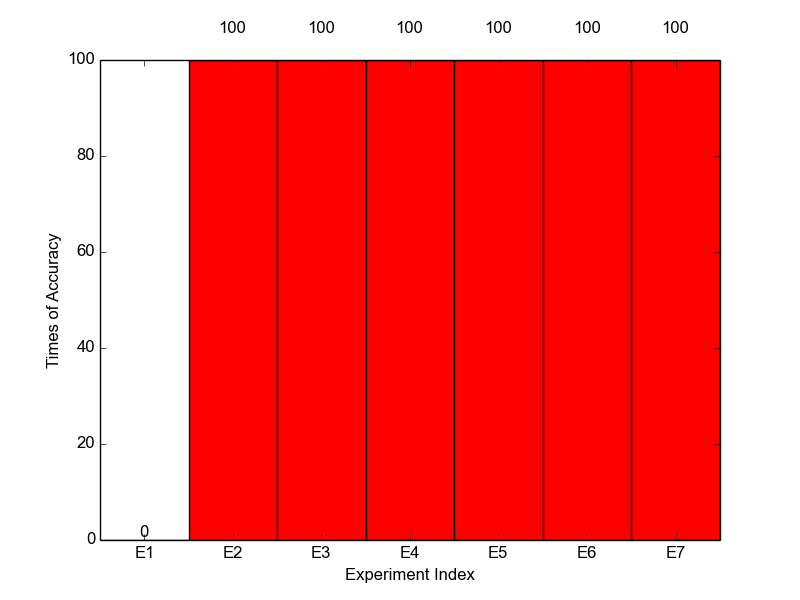
\includegraphics[scale=0.7]{Figures/accuracy_pecent_result8_mixture.png}
\caption{Accuracy analysis for experiments considering a mixture of amino acids with candidates from $0^{\circ}$ to $80^{\circ}$ on $\theta$ for each amino acid}  \label{fig:5.1}
\end{figure}

The experiment set is ran for 100 times, the result is shown in 
Figure \ref{fig:5.1}. In Experiment 2, the return composition of the LP model constructed by using Raman spectral information meets the target composition 100 times. This means that within this set of experiments, Raman is sufficient to obtain the correct composition of the target spectra. Moreover, the accuracy is 100\%. \\

Experiment 3 is the LP model constructed by using SFG spectral information. Its accuracy is 100\% as well as shown in Figure \ref{fig:5.1}. This indicates that SFG spectral information is as abundant as Raman for this set of experiments. . \\

Experiment 4, Experiment 5, Experiment 6, and Experiment 7 each contains either spetral information of Raman, or SFG, or both. Therefore, the corresponding LP model can help to get target composition with the same accuracy as Experiment 2 and Experiment 3. \\

The only exception is Experiment 1. The accuracy is not as high as the other experiments. The accuracy of LP model constructed using IR spectral information is $0$. The low performance can be caused by the insufficient spectral information of IR. \\
%This makes us wonder how come the performance of the LP model that merely use IR spectra be so low? And even if the performance is low, can we still extract any valuable information that indicates IR could still be useful in some cases? \\

When this experiment set is re-run 100 times, only Experiment 1's returned composition is analyzed and focused. In each run, IR $x$ and $z$ polarized spectra are plotted both by the returned composition and the target one. The result is these two polarizations' spectra conducted by the two different compositions are almost identical to each other in every run. For example, a random run is picked, then the two polarizations' spectra are plotted in Figure \ref{fig:5.2}. The spectra plotted by the return composition are identical to the ones plotted by the target composition. This indicates that the optimum composition returned by the LP model conducted with only IR spectral information has achieved its best in obtaining a composition that best fit the target spectra. 
%However, with limited information, the LP model cannot further distinguish the candidates, therefore, make it impossible to obtain an even more accurate composition. Moreover, because our candidates for each amino acid are quite similar to each other by just looking at the spectra. It is very possible that there are more than one possible compositions can perfectly re-construct the target spectra.  Therefore, we would need more constraints to refine our candidates' selection for the target composition. 

(TODO: rewrite or remove this paragraph) Comparatively, SFG has three unique polarizations, and Raman has four unique polarizations. From each projection's spectrum, we evenly select 200 data points. This means that one more projection will bring in 200 more constraints or 400 more (if we take the absolute sign off) constraints to the LP model. This would make a huge difference in LP model, in term of further refining the candidate selection in target composition. However, it is still too early for us to say that Raman has more coordination information because it has four unique polarizations. Because for Raman's any polarization, the spectrum of candidate with $\theta$ equals to one degree is identical to the one of candidate with this $\theta$ degree's complementary. For example, the Raman spectra for candidate with $\theta$ of $10^{\circ}$, is the same as candidate with $\theta$ of $170^{\circ}$. And for IR, it is the same case. Only SFG tells the differences between these two degrees, as the spectra for candidate with $\theta$ of one degree is symmetric to its complementary along wavenumber. \\

\begin{figure}[!ht] 
\centering
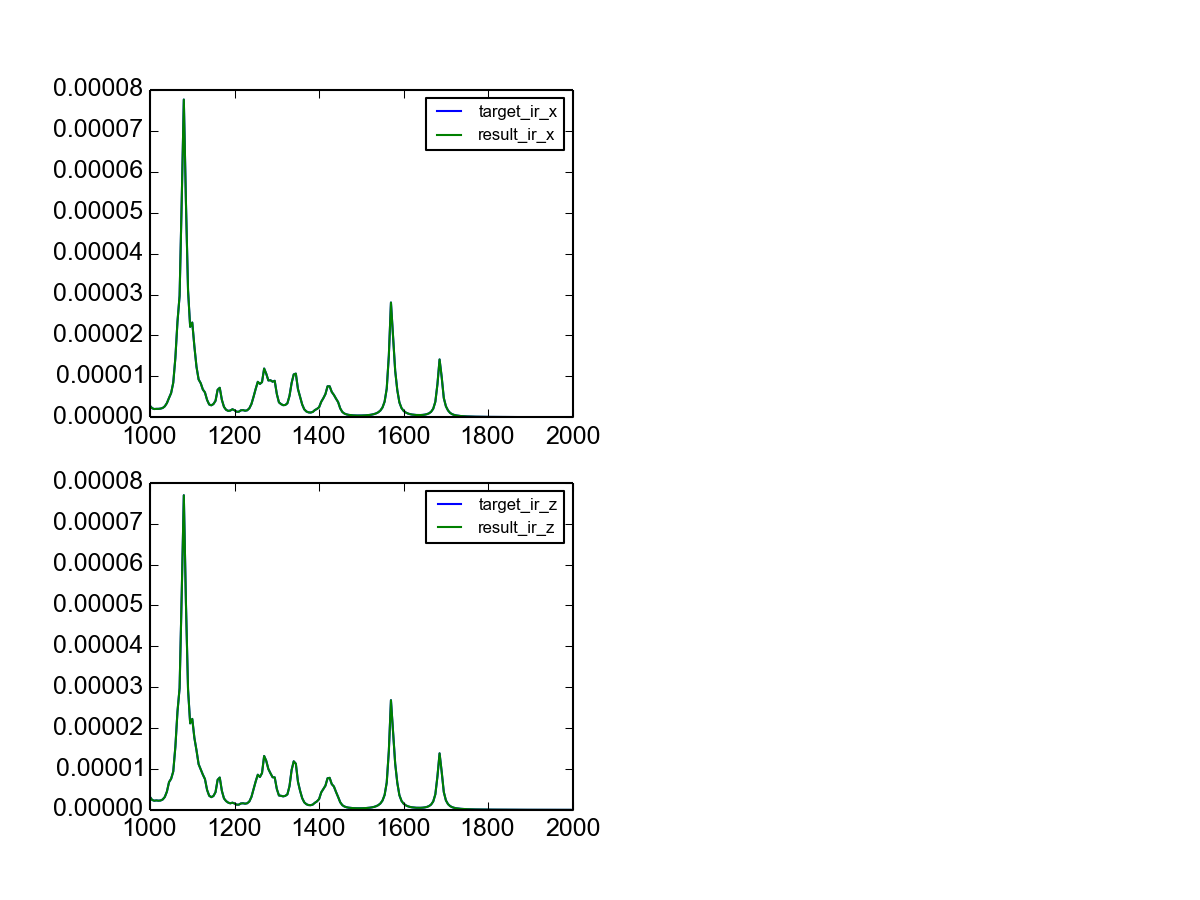
\includegraphics[scale=0.7]{Figures/result_target_plotting_ir16.png}
\caption{IR Spectra Plotted by Result Composition and Target Composition. TODO: add residual graph} \label{fig:5.2}
\end{figure}

%This shows that with the information that IR spectra have, it is not sufficient to abstract the orientation distribution of the mixed molecules at surface in this case.

%However, Raman or SFG only is good enough to obtain the desire result.

To further study the capacity of the LP models built for the mixture of molecules,the candidate pool is expanded from $0^{\circ}$ to $180^{\circ}$ in terms of the $\theta$ value. Therefore, each amino acid has 18 candidates. In total, there are 108 candidates in the mixture. The same set of experiments in Table \ref{tab:5.1} is used. The only difference is randomly select one candidate from 18 candidates, instead of 9. All 108 candidates' IR, Raman and SFG spectra need to be generated. Figure \ref{fig:5.3} illustrates the results obtained in $100$ runs. The accuracy in Experiment 1 is still low. This is not surprising as the complexity of the candidates has increased. Moreover, IR spectra for candidate with $\theta$ of one degree is identical to the one with $\theta$ of this degree's complementary, as shown in Figure \ref{fig:5.7}. This also increases the difficulty for the LP model constructed by using IR spectral information to return the target composition. \\
%Then we run the same group of experiments in Table \ref{tab:5.1} 100 times. The only differences are in the general setting. For target composition for each experiment group, we need to randomly select one candidate from 18 candidates, instead of 9. What's more, we need to 108 candidates' IR, Raman and SFG spectra. The goal is to study which experiment in Table \ref{tab:5.1} will give us the highest accuracy with current candidate pool. In return, we have Figure \ref{fig:5.3} showing the experiment result. 

\begin{figure}[!ht]
\centering
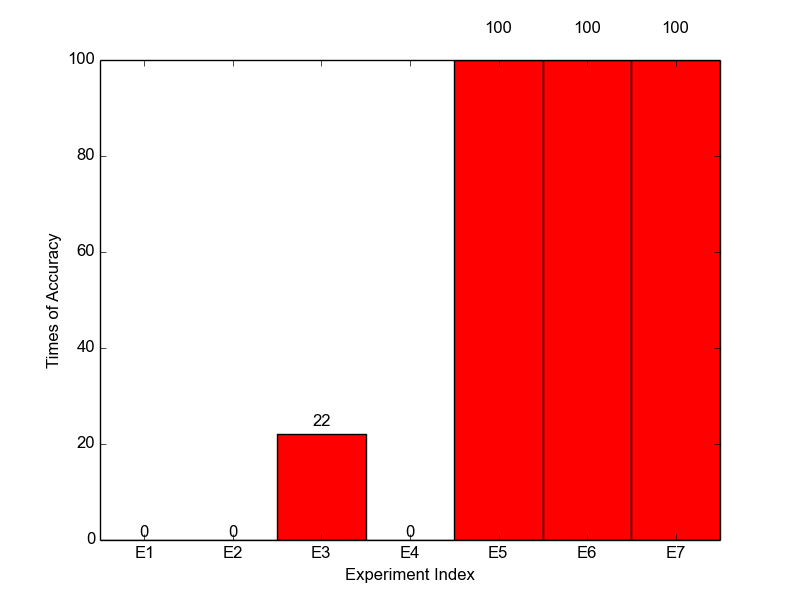
\includegraphics[scale=0.7]{Figures/accuracy_pecent_result10_mixture.png}
\caption{Accuracy analysis for experiments considering a mixture of amino acids with candidates from $0^{\circ}$ to $180^{\circ}$ on $\theta$ for each amino acid} \label{fig:5.3}
\end{figure}

However, it should be noticed that the accuracy for Experiment 2 has dramatically dropped. This is because the Raman spectra for one candidate with $\theta$ on one degree is identical to the one with this degree's complementary. Further explanation  is provided in Chapter \ref{ch:6} . \\

Also in Figure \ref{fig:5.3}, the accuracy for Experiment 3 is no longer high neither. After increasing the number of amino acid candidates from 9 to 18, the complexity of the corresponding LP model has increased. From each projection, 200 data points are selected from both the target and the candidates' spectra. Therefore, while the number of constraints is the same as before, the number of candidates are twice bigger than before. Although the added candidates' SFG spectra are symmetric along wavenumber which may greatly increase the uniqueness of the candidates. The spectral information is still insufficient to converge the composition to the target one. \\
% in the LP model, the objective function here is to minimize the sum of each data point's absolute subtraction between the target spectra and the one generated by candidates' spectra and return composition. Because of the nature(!!!need to expand a bit), composition return by E3's LP model can be far off the target one in the solution dimension if we do not have enough constraints.\\

%The reason for E4 to have low accuracy could be the same as E2. Even combining IR and Raman, there is no way for us to distinguish the candidates that with $\theta$ and the one with this degree's complementary, for each amino acid. We will compare the return compositions of E2 and E4 to see if there is any improvement after combining IR to Raman.\\

The good result starts to emerge when using the combinations of IR and SFG or Raman and SFG. Figure \ref{fig:5.3} shows that Experiment 5, Experiment 6, Experiment 7 all have 100\% accuracies. This phenomenon can be explained as follow: SFG helps to distinguish a candidate from its complementary on $\theta$ value. The extra spectral information coming from IR or Raman helps to further refine the LP model, which can then converge the return composition to the target one. \\
%This may not be hard to explain even in the first glance, when you combine IR with SFG, we have IR's 2 projection and SFG's 3 projection spectra. From SFG, we have information to distinguish from a candidate and its complementary $\theta$ degree. With the help of IR, we have enough information to construct the constraints in the LP model. Let along mentioning the combination of Raman and SFG, as Raman has 4 projection spectra where we can extra more data points to further refine the model. \\

Although the accuracy in Experiment 2 is low when each amino acid's candidates spread from $0^{\circ}$ to $180^{\circ}$ on $\theta$. There are still some noticable result in the return composition: for each amino acid, the percentage assigned to it is correct; however, the candidate presented may be the one with the correct degree, or the one with the correct degree's complementary. For example, a random run is selected. Figure \ref{fig:5.4} displays the target composition and Figure \ref{fig:5.5} displays the return composition of Experiment 2. Figure \ref{fig:5.6} is the return composition of Experiment 6. From the three figures, when extracting the non-zero values to generate a list, the three lists are the same. However, when overlapping Figure \ref{fig:5.4} with Figure  \ref{fig:5.5}, the position of each non-zero value is not identical. For example, value of $0.299586$ appears at $\theta$ of $150^{\circ}$ for Valine in Figure \ref{fig:5.4}. In Figure \ref{fig:5.5}, it appears at $\theta$ of $30^{\circ}$ for Valine. Same for value of $0.021196$, $0.00662804$, $0.000642609$, and $0.00789$. The LP model of E2 fails to tell which candidate is the exact one between the correct one and its complementary on $\theta$'s degree. This observation is a general case across all the experiment groups. From Experiment 6, as long as the spectra data from SFG is plugged into the LP model, the return composition is the same as the target one. \\


\begin{figure}[!ht] 
\centering
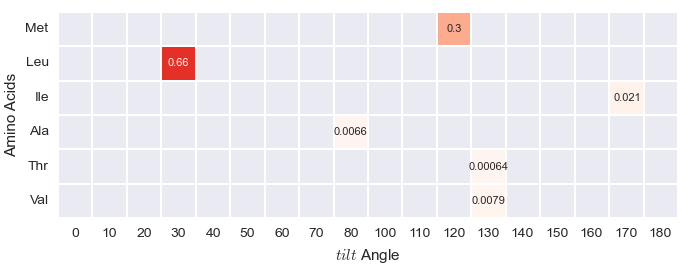
\includegraphics[scale=0.4]{Figures/mixture_target_composition_for_one_run_theta_0_180.png}
\caption{Target Composition for One Run of Mixed Amino Acids with $\theta$ Expanded from $0^{\circ}$ to $180^{\circ}$} 
\label{fig:5.4}
\end{figure}

\begin{figure}[!ht] 
\centering
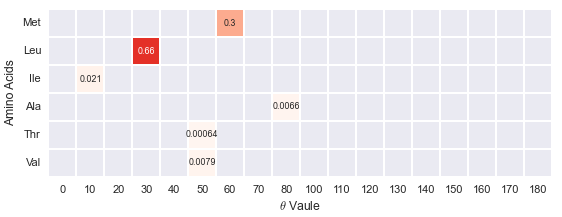
\includegraphics[scale=0.4]{Figures/mixture_return_composition_of_E1_for_one_run_theta_0_180.png}
\caption{Return Composition of Experiment 2 for One Run of Mixed Amino Acids with $\theta$ Expanded from $0^{\circ}$ to $180^{\circ}$ on $\theta$} 
\label{fig:5.5}
\end{figure}

\begin{figure}[!ht] 
\centering
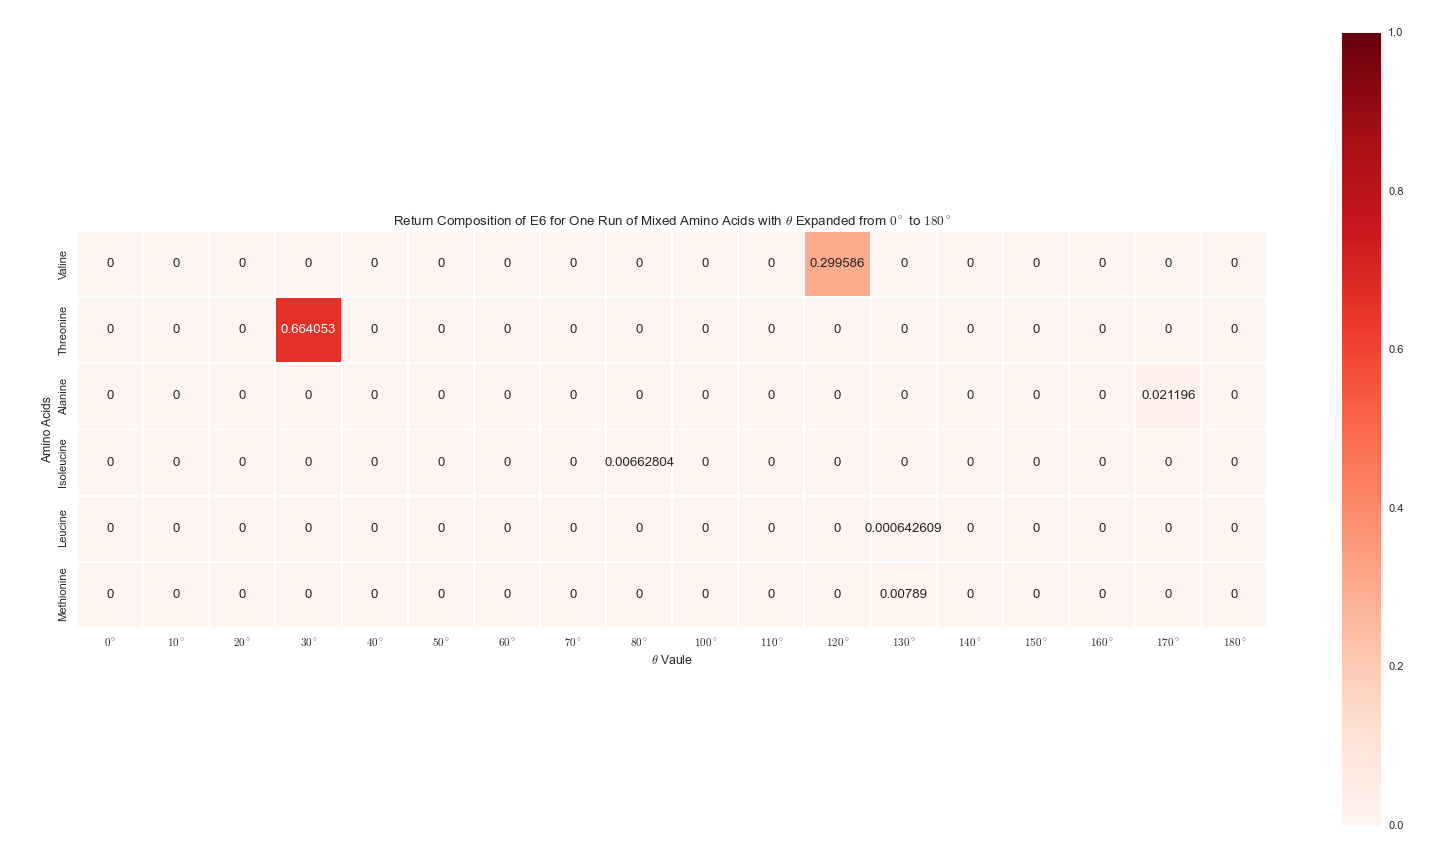
\includegraphics[scale=0.4]{Figures/mixture_return_composition_of_E6_for_one_run_theta_0_180.png}
\caption{Return Composition of Experiment 6 for One Run of Mixed Amino Acids with $\theta$ Expanded from $0^{\circ}$ to $180^{\circ}$ on $\theta$} 
\label{fig:5.6}
\end{figure}

%We randomly take one group of experiment run as an example, Array \ref{eqn:5.1} is the target composition that we generated randomly. And Array \ref{eqn:5.2} is the return composition of E2, Array \ref{eqn:5.3} is the return composition of E6. When comparing Array \ref{eqn:5.1} with Array \ref{eqn:5.2}, if we take the percentage value of each existing candidate in the target composition and the composition returned by E2, the two arrays are identical. However, what's different is the existing candidate for each amino acid may not be correct. For example, in target composition, we have 0.299586 of candidate with $\theta$ of $120^{\circ}$ for methionine, but the one return by E2, has 0.299586 of candidate with $\theta$ of $60^{\circ}$ for methionine. $60^{\circ}$ and $120^{\circ}$ are complementary to each other, which means the Raman spectra for these two candidates of methionine are identical. E2's LP model may take each one of them as an existing candidate in the return composition, and this may not be surprising. In the result, it is the same case for isoleucine(ile), alanine, threonine and valine. The LP model of E2 fails to tell which candidate is the exact one between the correct one and its complementary on $\theta$'s degree. This observation is a general case across all the experiment groups. What's more, from E6, we know as long as we plug in the spectra data from SFG into our LP model, we can obtain the correct composition same as the target one. \\

From the above analysis, Experiment 2 appears the ability of limiting the number of candidates to $2$ for each amino acid. These two candidates are complementary on $\theta$ degree, with one of them to be the correct one for the target composition. The return composition of Experiment 4 is the same as the one of Experiment 2, which means IR spectra information is not helping in this case. Spectral information from SFG is needed in order to study the cases that having $\theta$ expanded from $0^{\circ}$ to $180^{\circ}$.\\

%Experiment 2: the LP model that constructed by using only four projections of Raman spectra does not contain enough information any more for the current case. 

%Experiment 3: The information coming from SFG three projection is not completely sufficient, however, it is much better than IR or Raman. The underline reason is actually quite obvious, because the IR spectrum for $\theta = 0^{\circ}$ is the same as the one for $\theta = 180^{\circ}$, so as for Raman, the spectra of $\theta = 0^{\circ}$ and $\theta = 180^{\circ}$ are identical at every projection. Contrarily, the SFG spectra for them are symmetric. The following three pictures display Alanine's IR z projection, Raman zz projection and SFG zzz projection spectra. As shown, the IR and Raman spectra for theta with 0 degree and 180 degree are same, but for SFG, their are symmetric.

\begin{figure}[!ht] 
\centering
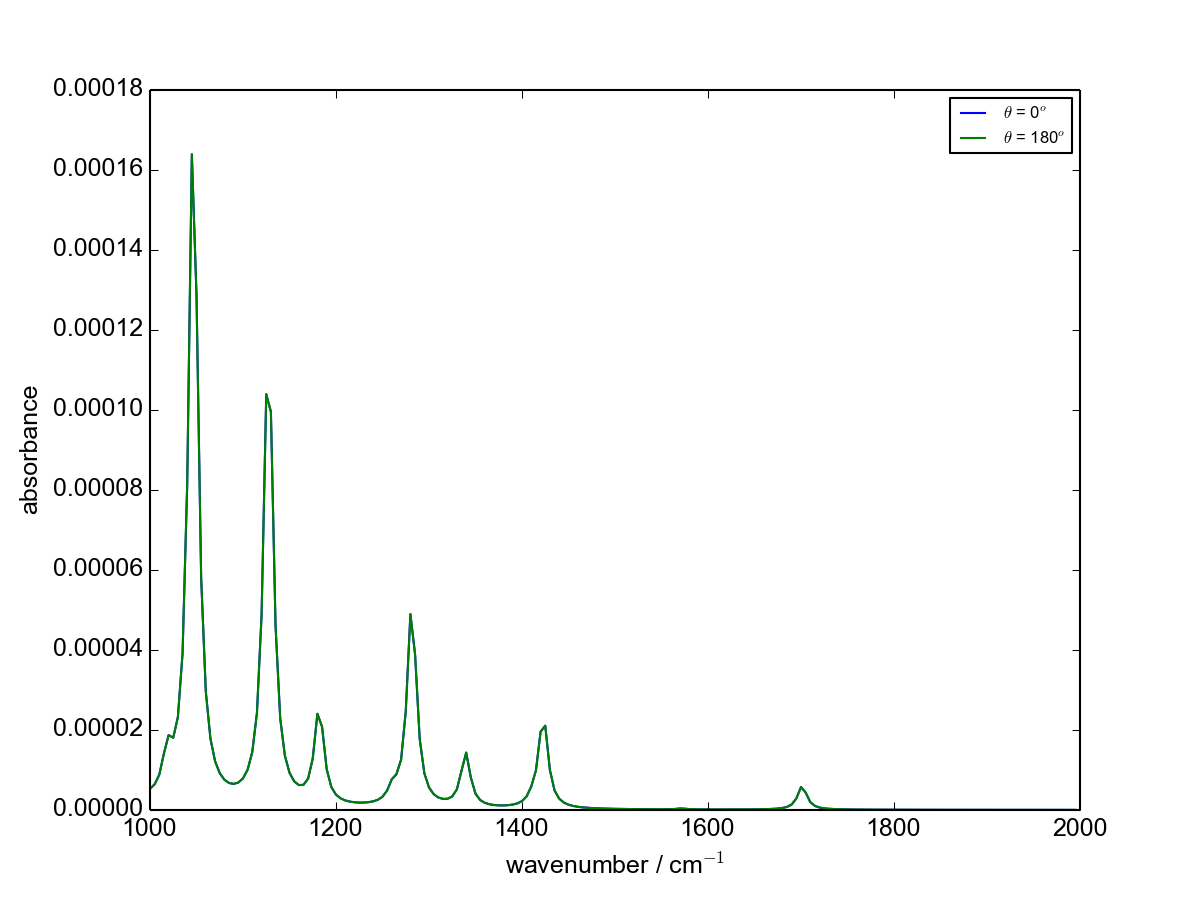
\includegraphics[scale=0.7]{Figures/Ala_candidates_plotting_ir_z_2.png}
\caption{IR z projection spectrum for Alanine Candidate with $\theta$ of $0^{\circ}$ is identical to Alanine Candidate with $\theta$ of $180^{\circ}$} \label{fig:5.7}
\end{figure}

\begin{figure}[!ht] 
\centering
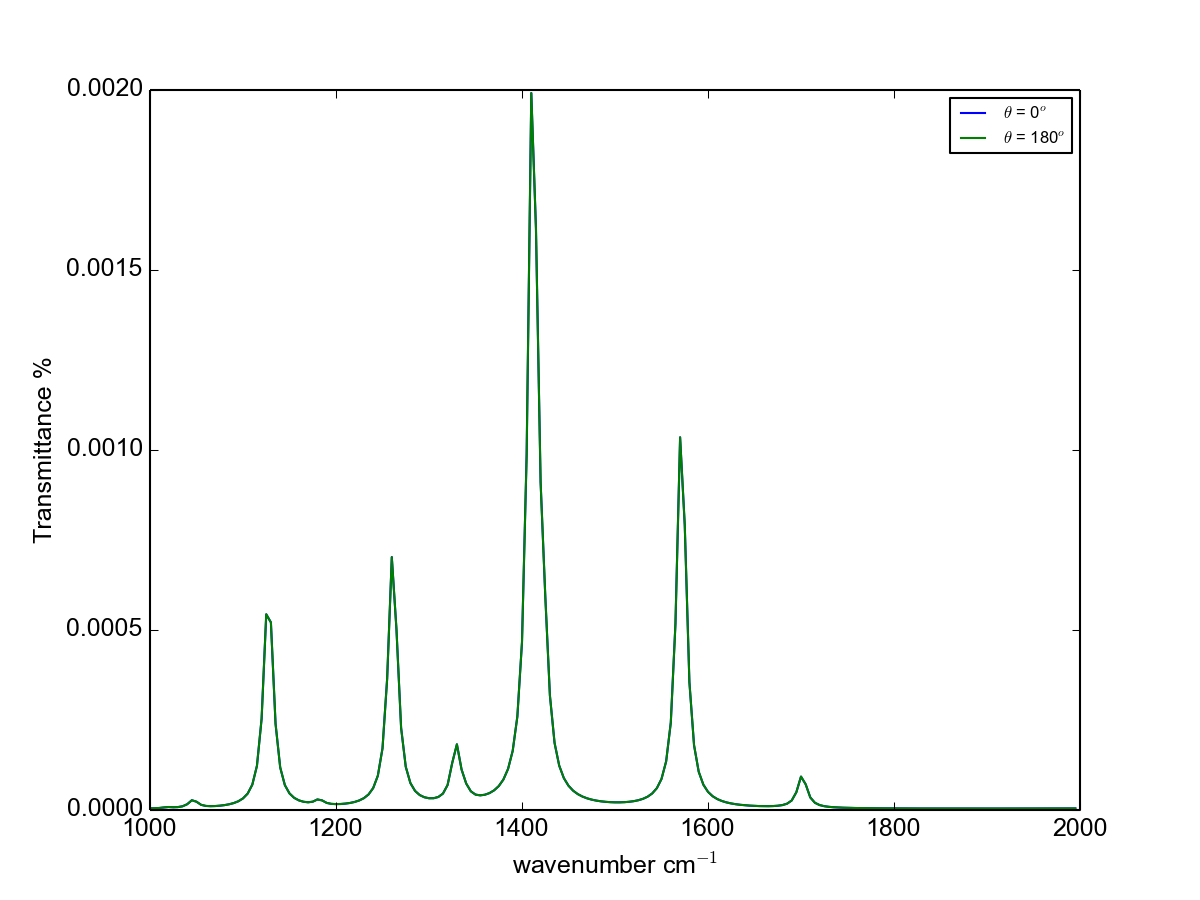
\includegraphics[scale=0.7]{Figures/Ala_candidates_plotting_raman_zz_2.png}
\caption{Raman zz projection spectrum for Alanine Candidate with $\theta$ of $0^{\circ}$ is identical to Alanine Candidate with $\theta$ of $180^{\circ}$} \label{fig:5.8}
\end{figure}

\begin{figure}[!ht] 
\centering
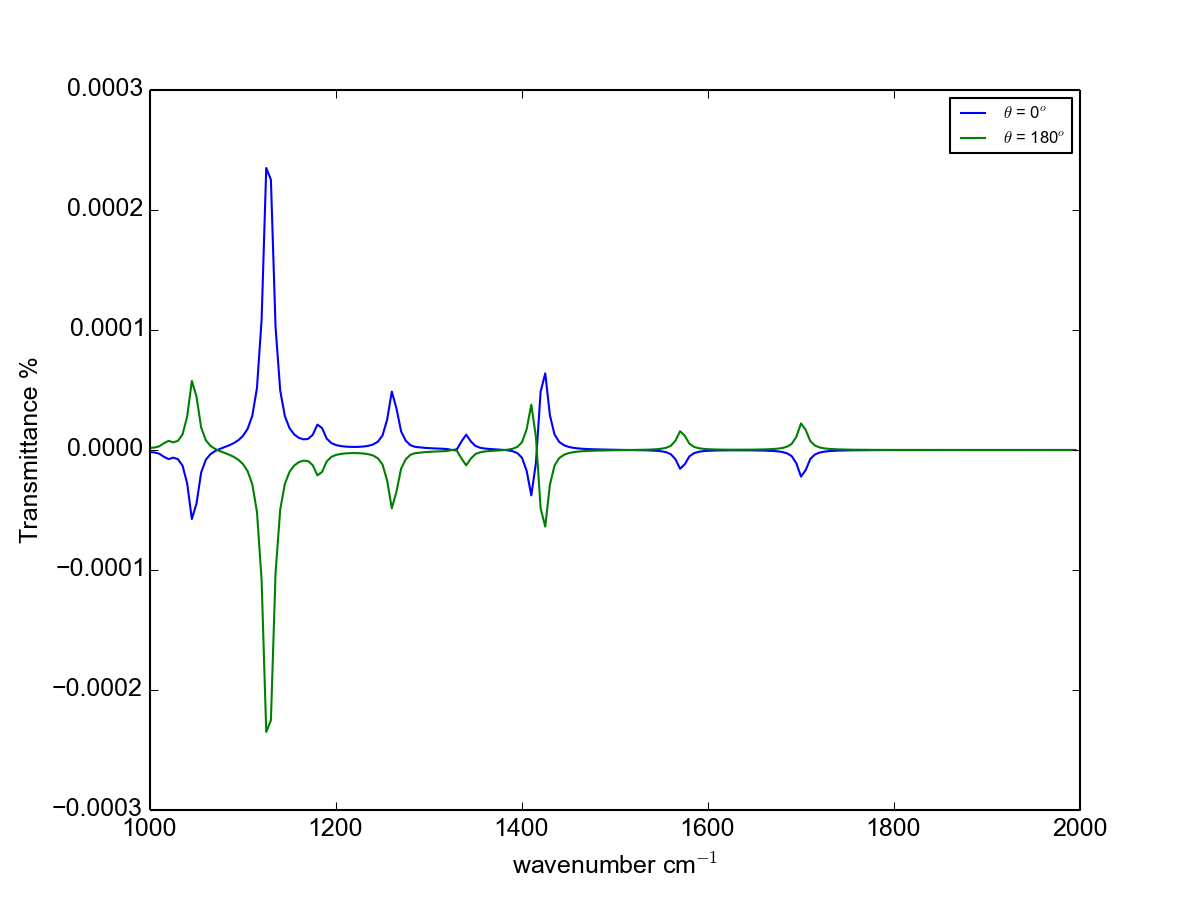
\includegraphics[scale=0.7]{Figures/Ala_candidates_plotting_sfg_zzz_2.png}
\caption{SFG zzz projection spectrum for Alanine Candidate with $\theta$ of $0^{\circ}$ is not identical to Alanine Candidate with $\theta$ of $180^{\circ}$, but symmetric along wavelength} \label{fig:5.9}
\end{figure}
